\subsection{Block Diagram}
\begin{figure}[h]
    \centering
    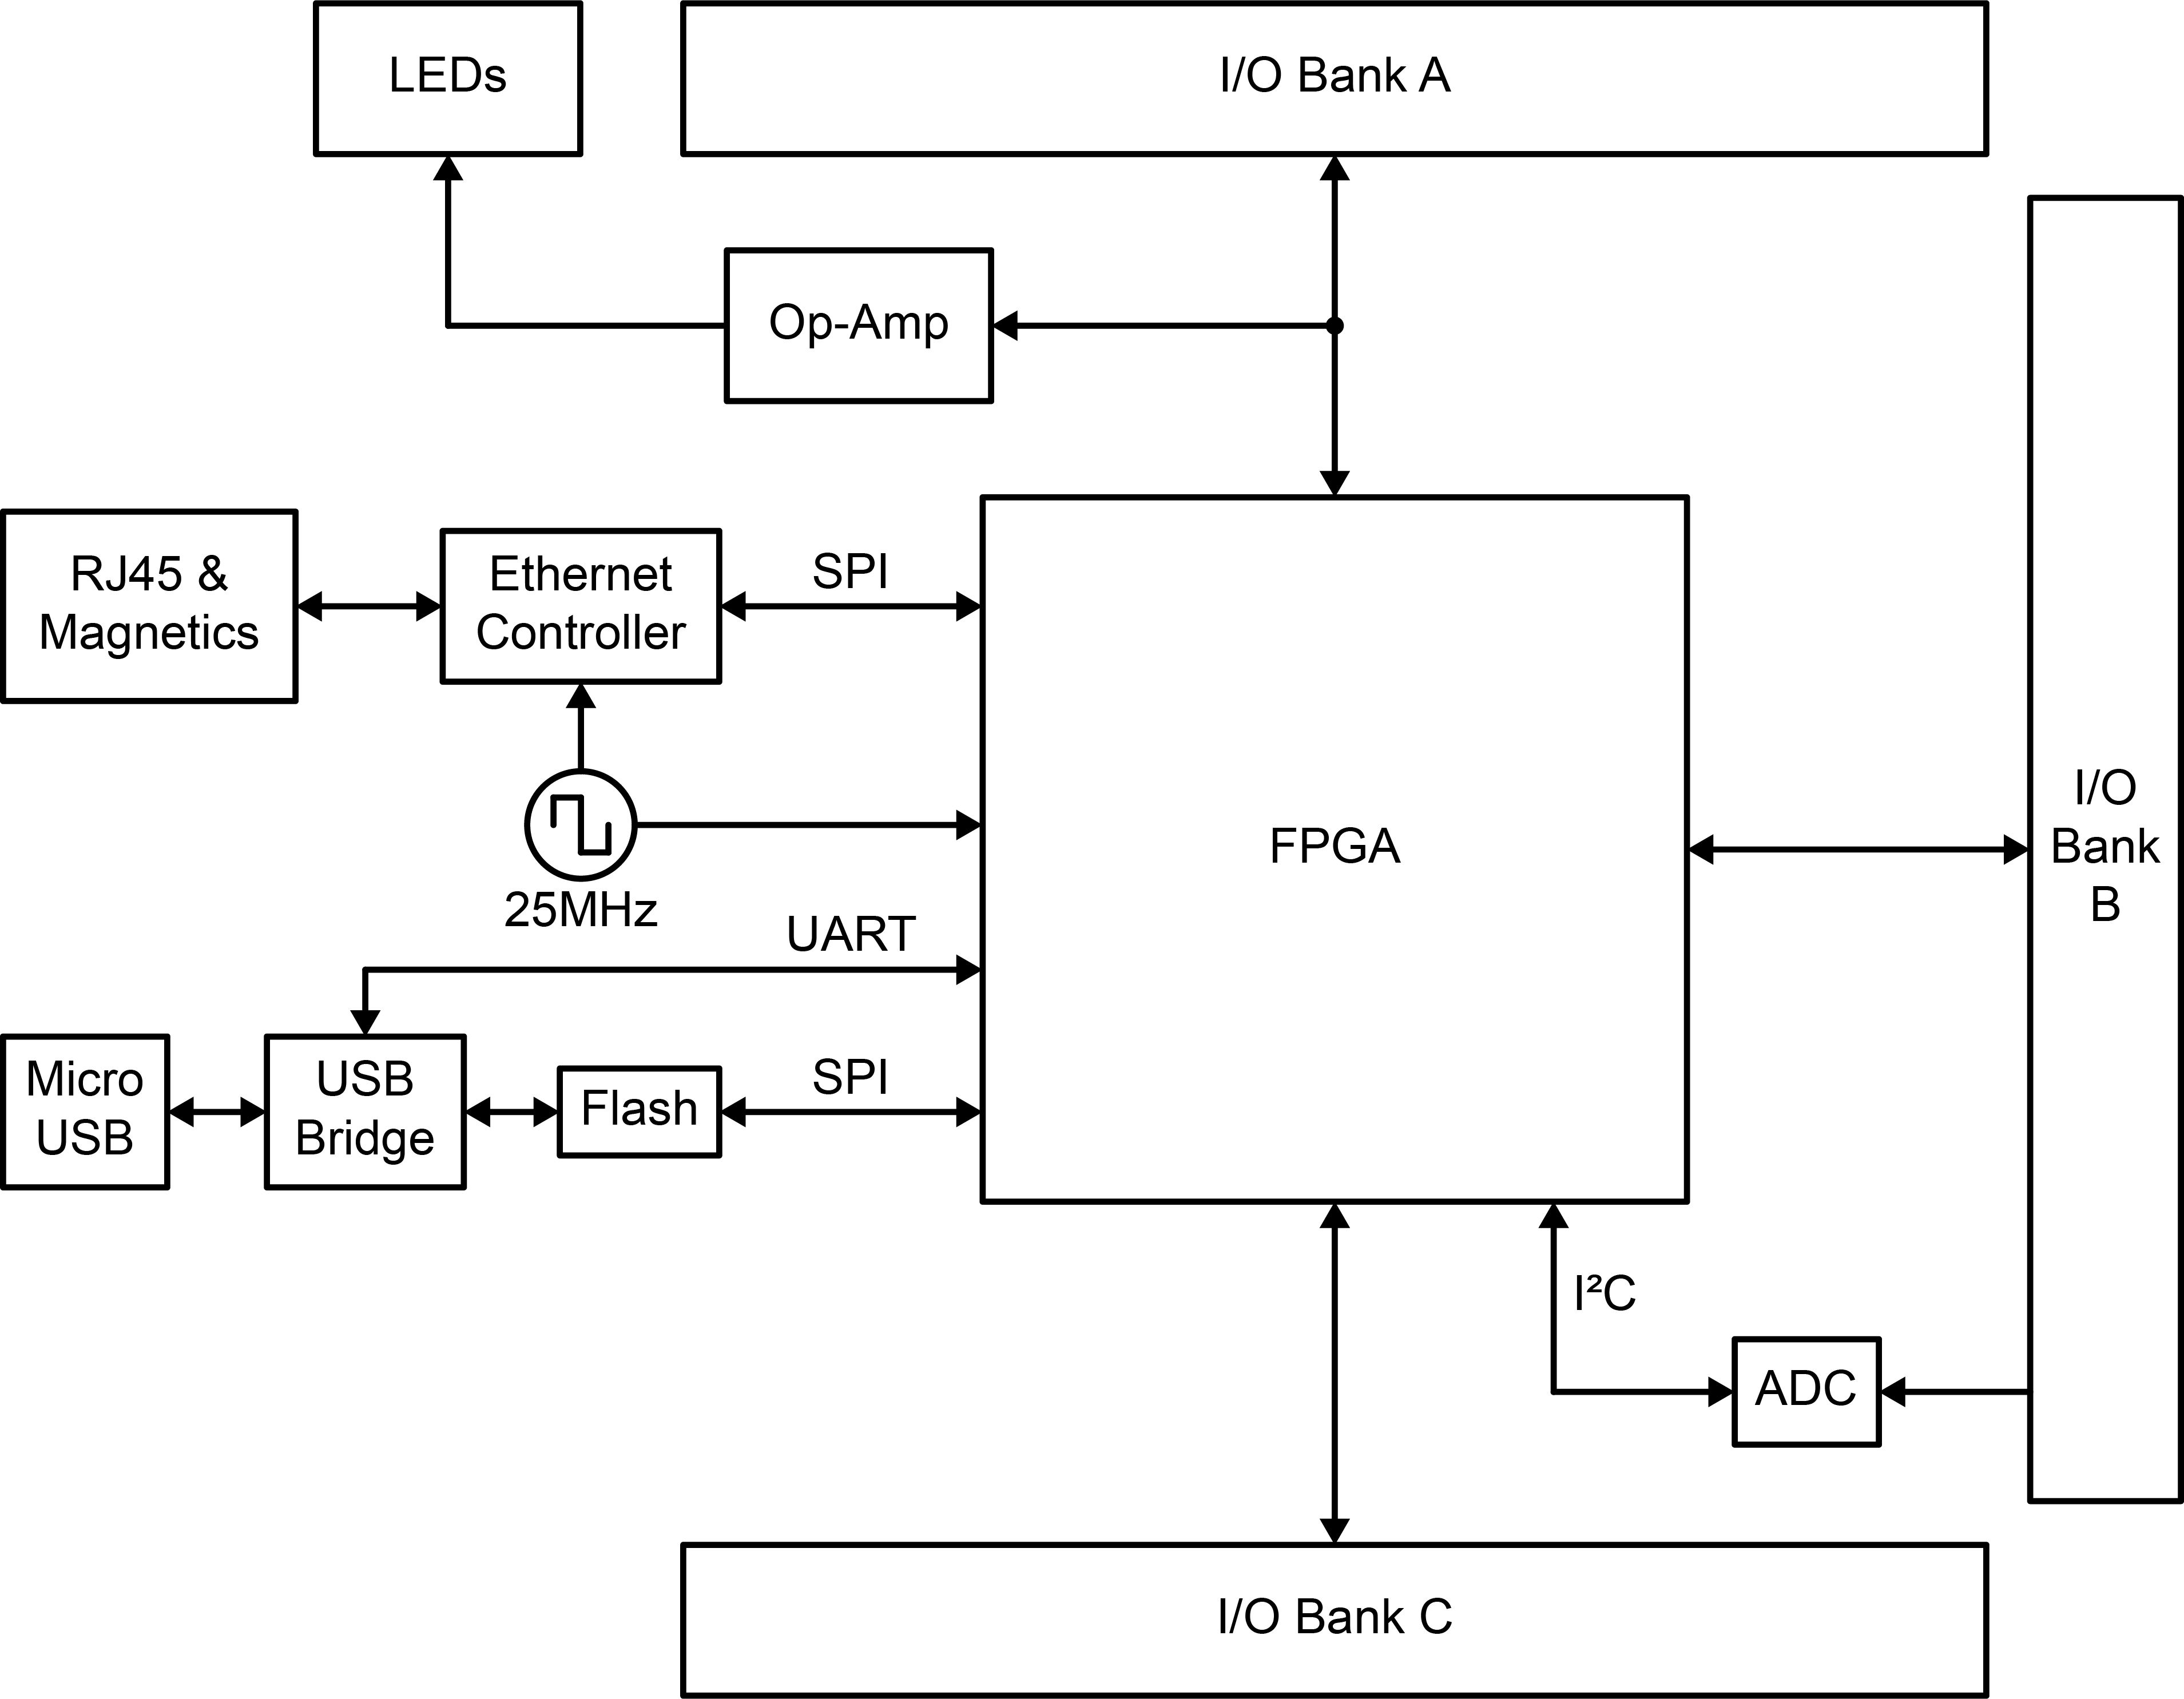
\includegraphics[width=9.5cm]{assets/block-diagram.png}
    \caption{Block Diagram}
\end{figure}

\subsection{FPGA Configuration} \label{section:fpga-config}
The FPGA can be configured using Lattice Semiconductor's iCEcube2 Design Software and Diamond Programmer. iCEcube2 is used to generate the bitstreams, while Diamond Programmer is used to flash the bitstreams on to the FPGA. For guides on using these tools, see both the \href{https://docs.thetamachines.com/hardware/disco-boards/eth4k/icecube2-guide}{\textit{iCEcube2 Guide}} and the \href{https://docs.thetamachines.com/hardware/disco-boards/eth4k/diamond-programmer-guide}{\textit{Diamond Programmer Guide}} available at \url{https://docs.thetamachines.com}.

\subsection{USB Bridge}
The FTDI FT2232H USB Bridge is used for both programming the FPGA and communicating over UART. Information on how the UART connects to the FPGA can be found in \autoref{section:internal-connections}. 

\textbf{Caution:} Modifying the FT2232H's firmware can permanently brick the ETH4K.

\subsection{Ethernet Controller}
The board integrates the WIZnet W5500 Ethernet controller, enabling network communication without the need to implement TCP/IP logic within the FPGA. This simplifies and shrinks designs while still offering robust communication. The W5500 has an embedded 10BASE-T/100BASE-TX PHY and supports TCP, UDP, ICMP, IPv4, ARP, IGMP, and PPPoE.

The W5500 communicates with the FPGA over a SPI bus with an additional reset pin and interrupt pin (see \autoref{section:internal-connections} for connection information).

\newpage

\subsection{Analog to Digital Converter}
The ETH4K integrates the Texas Instruments ADS1015. This 12-bit ADC has four analog inputs (A[3:0]). It accepts signals between 0V and 3.3V and has a programmable sampling rate from 128 to 3,300 samples per second.

The ADS1015 also integrates a digital comparator capable of issuing an alert when the input signal falls outside of some programmable threshold. 

\subsection{Flash Memory}
The ETH4K is equipped with the Winbond W25Q80DV. This serial NOR flash module has 1MiB (1,048,576 bytes) of non-volatile memory. The FPGA must be programmed with at least one bitstream, which takes up 135,183 bytes. All remaining space may be used for general purpose storage. The FPGA communicates with the flash module over a four-wire SPI bus. These pins are not released to the user as GPIO until 49 clock cycles after the FPGA has been configured. See \autoref{section:internal-connections} for connection information.

\textbf{Caution:} Be careful not to overwrite the FPGA bitstream when writing to this memory. If this happens, the device must be reprogrammed. 

\subsection{Multiple Bitstreams} \label{section:multiple-bitstreams}
% Be sure to talk about both cold and warm booting (as well as normal configuration)
The iCE40HX4K FPGA supports several programming configurations. By default, the device is programmed with a single bitstream. If you wish to flash multiple bitstreams, then two configuration modes are supported: Cold Boot mode and Warm Boot mode. Both of these modes can be configured in the Diamond Programmer software discussed in \autoref{section:fpga-config}. Up to four bitstreams are supported.

In Cold Boot mode, the CBSEL[1:0] pins are monitored during startup. These pins determine which of the bitstreams will be used to program the FPGA. The CBSEL[1:0] pins are discussed further in \autoref{section:CBSEL-pins}.

In Warm Boot mode, the FPGA controls which bitstream is loaded through the SB\_WARMBOOT primitive. The bitstream is selected through the internal S[1:0] signal ports, and the BOOT port triggers the FPGA to restart into the selected bitstream. More information on the SB\_WARMBOOT primitive can be found in the \href{https://www.latticesemi.com/view_document?document_id=52206}{\textit{iCE40 Technology Library}} technical note published by Lattice Semiconductor.

For more information on both Cold Boot and Warm Boot modes, see the \href{https://www.latticesemi.com/view_document?document_id=46502}{\textit{iCE40 Programming and Configuration}} technical note published by Lattice Semiconductor.

\newpage